\documentclass[10pt]{exam}
\usepackage[hon]{template-for-exam}
\usepackage{multicol,graphicx,pgfplots}
\pgfplotsset{compat=1.18}

\title{Friction Stations}
\author{Rohrbach}
\date{\today}

\begin{document}
\maketitle


\section{Book Reading} \label{book}

Read {\bf Section 5.1: Friction (pp. 198ff)} in OpenStax \emph{College Physics} to answer these questions.

\begin{enumerate}
  \item 
    What is friction?
    \vs

  \item
    What's the difference between \emph{kinetic friction} and \emph{static friction}?  Which is stronger?
    \vs

  \item 
    As you push a crate harder and harder, what happens to the force of friction before the crate starts to move?
    \vs

  \item
    What causes friction?
    \vs

  \item 
    Write down the equations for static friction and kinetic friction:
    \vs
  

  \item 
    Study Table 5.1. You should notice that $\mu_s>\mu_k$ for every pair of surfaces.  Given what you've read, why does this make sense?
    \vs

  \item 
    Study Figure 5.5. Why does it make sense that larger normal force leads to higher amounts of friction?
    \vs
\end{enumerate}

\pagebreak


  


\pagebreak
\section{Vernier Force Probes} \label{vernier}

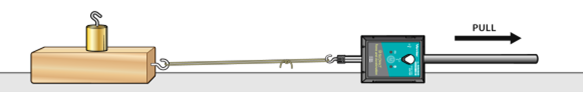
\includegraphics[width=8cm]{friction-lab.PNG}

\begin{questions}
  \question
    Make sure your Force Sensor is set to $\pm 10$ N.

  \question 
    Before you collect data, practice pulling the block and masses with the force sensor using a straight-line motion. Slowly and gently pull horizontally with a small force. \emph{Very gradually,} taking one full second, increase the force until the block starts to slide, and then keep the block moving at a constant speed for another second.




  \question 
    Zero the force sensor before collecting data.

    \begin{minipage}[b]{10cm}
      \begin{parts}
        \part Place the force sensor on a flat surface so the working axis is horizontal.
        \part With the force sensor axis held horizontally and no force applied, click or tap the Force meter at the bottom right of the screen and choose Zero.
      \end{parts}
      \vspace{6em}
    \end{minipage}
    %
    \hfill
    %
    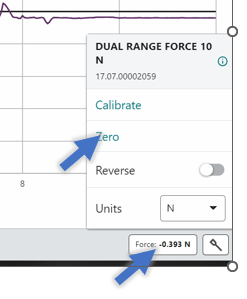
\includegraphics[width=4cm]{zero}
      


  \question
    Take your first set of data
  
    \begin{parts}
      \part   
        Stack 600 g (three 200-g weights) on top of the block.  Spread the weights evenly on the block.	
      \part
        Hold the force sensor in position, ready to pull the block, but with tension in the spring.
      \part 
        Click {\bf Collect} to start data collection. Wait a moment, then pull the block, taking care to increase the force gradually.
      \part
        Inspect your graph. It should reflect the desired motion, including pulling the block at constant speed once it begins moving. If it does not, start data collection and repeat the pulling process. 
      
      \part
        Sketch your graph below:
  
        \begin{tikzpicture}
          \begin{axis}[
            xlabel={\bf time},
            ylabel={\bf force},
            ymin=-5,
            ymax=5,
            xmin=0,
            xmax=4,
            ytick=\empty,
            xtick=\empty,
            axis y line = left,
            axis x line = center,
            height = 5cm,
            width = 15cm
          ]
          \end{axis}
        \end{tikzpicture}
      
    \end{parts}
  
   
  
  \question
    Explain what your graph shows and how it makes sense given what you learned in Station~\ref{book}.
    \vs

  \question
    Label the point on the graph where the block starts moving.  Also, label the section on the graph where there is static friction and kinetic friction.

  \pagebreak
  \question
    Click the graph to examine the data. The maximum value of the force occurs when the block started to slide. Click or tap the peak static friction force and record the value in your data table. \emph{Note: You can also adjust the Examine line by dragging the line.}
  
  \question
    Next you need to determine the average friction force while the block was moving at constant velocity.
  
  
      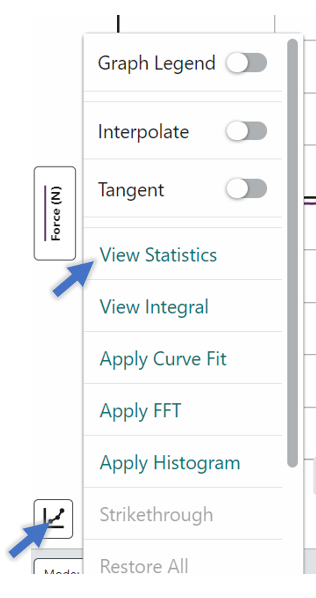
\includegraphics[width=4cm]{graph-tools}
      %
      \hfill
      %
      \begin{minipage}[b]{11cm}
        \begin{parts}
          \part 
            Select the data in the approximately constant-force region of the graph.
          \part
            Find the `Graph Tools' Icon at the bottom left of the screen then click {\bf View Statistics}.
          \part
            Record the mean force value in your data table.
        \end{parts}
        
        \vspace{1cm}
          
        \begin{tabular}{|l
          *3{|>{\centering\arraybackslash}m{1cm}}
          ||>{\centering\arraybackslash}m{1.5cm}|}
          \hline
            & Trial 1 & Trial 2 & Trial 3 & Average \\\hline
          Maximum Static Friction &&&&\\[2em]\hline
          Average Kinetic Friction &&&&\\[2em]\hline
        \end{tabular}

        \vspace{1cm}

      \end{minipage}
      


  \question
    Repeat Steps 10-12 for two more measurements and average the results to determine the reliability of your measurements. Record the values in the data table. 


  \question
    Which type of friction is stronger?  Does this match what you learned in Section~\ref{book}?
    \vs
  
\end{questions}

\pagebreak
\section{Spring Scales} \label{scales}

\begin{enumerate}
  \item 
    Hook up the spring scale to one of the blocks. Place 400 grams on top of the block.  Pull the block until it moves.  Pay particular attention to what happens to the reading on the scale just before it ``budges.''  Using what you learned in Section~\ref{book}, explain how this shows the difference between static friction and kinetic friction.
    \vs
    
  \item
    To measure the kinetic friction acting on the block, you need to pull the block across the table top at a constant velocity. While moving at a constant velocity, the scale will read the value for the kinetic friction.  Do this three times and average the values together.  Make sure to keep the 400 grams on top of the block

    \begin{tabular}{|l
      *3{|>{\centering\arraybackslash}m{.1\textwidth}}
      ||>{\centering\arraybackslash}m{.1\textwidth}|}
      \hline
      & Trial 1 & Trial 2 & Trial 3 & Average \\\hline
        Kinetic Friction &&&& \\
        (\emph{block is sitting flat}) &&&& \\\hline
    \end{tabular}


  \item \label{area-predict}
    The wood block has two surfaces it can slide over.  If you turn the block on its side you can measure the friction of a smaller surface area. Notice that the formula $f_k=\mu_kN$ has no surface area in the equation.  Given this fact, what do you think will be the result of sliding the block on its side? Will there be more friction, less friction, or the same amount of friction?
    \vs 

  \item 
    Let's test your prediction.  Turn the block on its side, make sure to stack the 400 grams on top, and measure the kinetic friction.

    \begin{tabular}{|l
      *3{|>{\centering\arraybackslash}m{.1\textwidth}}
      ||>{\centering\arraybackslash}m{.1\textwidth}|}
      \hline
      & Trial 1 & Trial 2 & Trial 3 & Average \\\hline
        Kinetic Friction &&&& \\
        (\emph{block is on its side}) &&&& \\\hline
    \end{tabular}

  \item 
    Evaluate your prediction from question~\ref{area-predict}.  Were you correct?
    \vs 
    
    
\pagebreak
  \item \label{weight-predict}
    Given what you learned in Section~\ref{book}, what do you think will be the result of adding weight to the block? Will there be more friction, less friction, or the same amount of friction?
    \vs 
  
  \item 
    Let's test your prediction.  

    \begin{tabular}{|c
      *3{|>{\centering\arraybackslash}m{.1\textwidth}}
      ||>{\centering\arraybackslash}m{.1\textwidth}|}
      \hline
        \bf Wood on table & Trial 1 &
                            Trial 2 & 
                            Trial 3 &  Average \\\hline
        Block + 200 g &&&& \\[1.5em]\hline
        Block + 400 g &&&& \\[1.5em]\hline
        Block + 600 g &&&& \\[1.5em]\hline
    \end{tabular}

  \item 
    Evaluate your prediction from question~\ref{weight-predict}.  Were you correct?
    \vs 



  \item \label{material-predict}
    What do you think will happen if you turn the block upside down so that the rubber side is facing down
    \vs 
  
  \item 
    Let's test your prediction.  

    \begin{tabular}{|c
      *3{|>{\centering\arraybackslash}m{.1\textwidth}}
      ||>{\centering\arraybackslash}m{.1\textwidth}|}
      \hline
        \bf Rubber on table & Trial 1 &
                              Trial 2 & 
                              Trial 3 &  Average \\\hline
        Block + 200 g &&&& \\[1.5em]\hline
        Block + 400 g &&&& \\[1.5em]\hline
        Block + 600 g &&&& \\[1.5em]\hline
    \end{tabular}

  \item 
    Evaluate your prediction from question~\ref{material-predict}.  Were you correct?
    \vs 


\end{enumerate}

\pagebreak

\section{Instructor Notes}

\begin{multicols}{2}

  friction depends on

  \vspace{4em}

  friction is indepenedent of

  \vspace*{4em}


  definition of the \emph{coefficient of friction}


  \columnbreak

     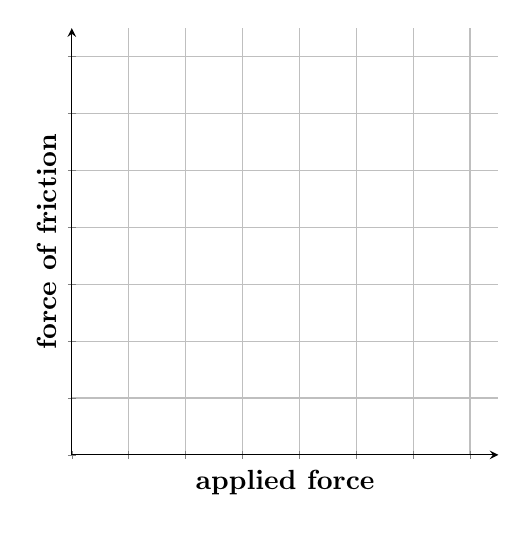
\begin{tikzpicture}
          \begin{axis}[
            xlabel={\bf applied force},
            ylabel={\bf force of friction},
            ymin=0,
            ymax=7.5,
            xmin=0,
            xmax=7.5,
            ytick={-10,10},
            xtick={-10,10},
            minor tick num = 19,
            grid=minor,
            axis y line = left,
            axis x line = bottom,
            height = 7cm,
            width = 7cm
          ]
          \end{axis}
        \end{tikzpicture}
  
\end{multicols}

\vspace{7em}

\paragraph{Example Problem}
A 75-kg bookcase is pushed across a carpeted floor.  The coefficient of static friction is 0.8 and the  coefficient of kinetic friction is 0.6.

\vspace{1em}
  \begin{parts}
    \part 
      How much force is required to start the bookcase moving?
      \vs
    \part 
      If that same force is continually applied to the bookcase after it starts moving, what will its acceleration be?
      \vs
  \end{parts}

\end{document}